\documentclass{llncs}
\usepackage{graphics}
\usepackage{graphicx}
\usepackage{amsmath}
\usepackage{amssymb}
\usepackage{algorithm}
\usepackage{algorithmic}
\usepackage{tikz}
\usepackage{hyperref}



\newtheorem{defin}     {Definition}
\newtheorem{theo}      {Theorem}
%\newtheorem{lemma}  {Lemma}
\newtheorem{cor}[theo]{Corollary}
\newtheorem{prop}      {Property}
\newtheorem{hyp}       {Assumtion}
\newtheorem{nota}       {Notation}
\newtheorem{meth}       {Method}
\newtheorem{ques}       {Question}
\newtheorem{rem}       {Remark}
\newtheorem{ex}       {Example}

\begin{document}

\mainmatter  

\title{Performance paradoxes in matching systems are not that rare}

\author{A. Busic$^1$, J.M. Fourneau$^{1,2}$, A. Lunven$^1$, S. Li$^1$ }

\institute{
$1$, INRIA ARGO, Paris, France \\
\email{ana.busic@inria.fr, antoine.lunven@ens-paris-saclay.fr, shu.li@inria.fr} \\
$2$  DAVID, Univ. Paris-Saclay, UVSQ, Versailles France\\
\email{Jean-Michel.Fourneau@uvsq.fr}
}
\maketitle
%%%%%%%%%%%%%%%%%%%%%%%%%%%%%%%%%%%%%%%%%%%%%%%%

\begin{abstract}
A Matching model describes the waiting times suffered by items before they match with other items 
and disappear immediately without service.  The matching relation is described by a compatibility graph. 
It is an easy representation of multiple types synchronizations 
between items. 
When we add an edge in the compatibility graph, one expect that the expected total number of items decreases. 
Unexpectedly this is not always true and there is a performance paradox. Extending previous results we show
new matching models with performance paradoxes which seems to be more frequent than one can expect. 
\end{abstract}


\section{Introduction} 


Following \cite{MaMo18} a Matching model is  a triple $( G, \Phi, \alpha) $ defined by 
\begin{enumerate}
\item a matching graph $G=(\cal{V},\cal{E})$ which is an undirected graph whose nodes in $\cal{V}$ are classes of items 
and whose edges in $\cal{E}$ models the allowed matching of items. $G$ is called the compatibility graph or the Matching graph. Upon arrival, an item is queued if there are not 
compatible items present in the system.

\item $\Phi$ is a matching policy. It states the couple of items which is chosen 
upon arrival when an arriving item matches one or more  items already waiting. Typical matching disciplines are First Come First Match (FCFM, an analog of First Come First Served in this approach) or Match the Longest Queue. 
Once they are matched, both items leave the system immediately (no need for service). 
\item a distribution of probability $\alpha$ to model the arrivals of items. Alternatively one can consider a collection of Poisson processes for
a continuous-time model. 
\end{enumerate} 
A matching occurs when two (or more) compatible items are present and it is performed 
according to the matching discipline. 

The general matching model proposed in \cite{MBMa21} and  \cite{MaMo18}
was considering a general undirected matching graph $G$ and it is assumed that the arrivals of items occur one at a time.
It is important to avoid the confusion with Bipartite Matching Model (see for instance  \cite{BGMa13}  and references therein) 
where the matching graph is bipartite
and   two items of distinct classes arrive at the same time. 

General matching models are easy to describe but they not so simple to analyze. 
Assuming independent Poisson arrivals of items, 
and FCFM discipline
the model is associated with an infinite Markov chain. 
A necessary condition of stability and a product form solution were proved in  \cite{MBMa21} and  \cite{MaMo18}
for these assumptions. 

Some of us have recently established that there exists some performance paradox for FCFM matching models \cite{CDFB21}. 
When one add  new edges in the compatibility graph, one may expect that the expectation of the total number of customers decreases. 
In \cite{CDFB21}, some examples were presented to 
show that it is not always the case and  a sufficient
condition for such a performance paradox to exist is proved. Thus, adding flexibility on the matching does not always result in a performance 
improvement. The example was based on an almost complete graph. In \cite{BCDF24}, 
the results have extended  
in many directions: all greedy disciplines instead of FCFM, and an infinite family of compatibility graphs. However
some questions remain about the compatibility graphs which lead to performance paradoxes. 
 
An application of Matching models  studied in the literature was the kidney 
exchanges \cite{KidneySite,Unve10,AJMa13}. 
The  kidney exchange arises when a healthy person who wishes to donate a kidney is 
not compatible (blood types or tissue types) with the receiver. Two incompatible pairs (or maybe more) can form a cyclic exchange, so
that each patient can receive a kidney from a compatible donor. %This application motivates one of the new results we develop in this paper. Indeed, in the kidney exchange problem the items may leave the system because of health problems. In the context of queueing theory this is noted as abandonment and the rates of such events is proportional to the number of items. This models do not fit in the assumptions of \cite{MBMa21} and  \cite{MaMo18}. Thus we develop new theoretical results to analyze some of them. 



The technical part of the paper is as follows. We begin in the next section with a short presentation
of performance paradoxes for Matching systems. Section 3 is devoted to a simple example built
for a compatibility graph with $5$ nodes which  was not considered previously. 
In Section 4, we also find some performance paradoxes for multi-graphs.% while in Section 5 we extend Matching models to add abandonment (with the Kidney exchange problem as a motivation) and we also find paradoxes in that case for a very simple compatibility graph. 
The objective of the paper is to  show arrival rates and compatibility graphs which 
exhibit performance paradoxes. The vector of arrival rates have been obtained 
through brute force inspection. Two numerical software 
based on the closed form solution for expectation of total number of items 
based on the independent sets 
have been developed for cross-validation and a simulator was also used during the validation process. 

\section{Performance Paradoxes in Matching Systems} 

Let $G=(\cal{V},\cal{F)} $ be the matching graph. Usually, nodes in $\cal{V}$ are also denoted as letters and  an 
ordered list of letters is  called a word. 
Assume that  $x$ is a letter from $\cal{V}$, $\Gamma(x) $ is the set of neighbors of $x$ in $G$. In this paper, 
we only consider FCFM matching disciplines even if some results on paradoxes have been established for 
the larger set of greedy disciplines \cite{BCDF24}.  In this paper, $\mathbb{E} [G, \alpha] $ will denote the 
expected number of items for compatibility graph $G$ and vector of arrival rates $\alpha$. 
Let $G$ be a graph and $a,b$ two nodes of $V$ such that $(a,b)$ is not an edge of $G$, 
we will denote as $G+e$, the graph $G$ where we have added edge $e=(a,b)$. 
Similarly,  $G-(u,v)$ where $(u,v)$ is an edge of $G$, is the graph obtained after removing edge $(u,v)$.
Finally, $\mathcal{I}$ will denote the set of Independent Sets of the compatibility graph.
  
\begin{theorem} [Product form for the steady-state distribution]\label{th:simple} \cite{MBMa21}
Assuming ergodicity, the steady state distribution for word $w$ is:
\[
\pi (w) = C \frac{\prod_{i=1}^{l(w)} \alpha_{w_i} }{\prod_{k=1}^{l(w)} \alpha(\Gamma(\{w_1,..w_k\}))},  
\]
where $l(w)$ is the length of word $w$, $w_i$ is the i-th letter of $w$, $\alpha (S)$ is 
the sum of the arrival rates for letters in $S$.
\end{theorem}

But it remains to compute the normalizing constant (i.e. $C$) and the expectation of the total number of items
 in the system: a difficult task as the state space of the Markov chain is infinite. 
Hopefully, close-form expressions have been obtained for these quantities. 
\begin{cor} [Expectation]\label{cor:exp} \cite{CDFB21}
For all independent sets $\mathcal{I} \in \mathbb{I}$, consider an ordered version of $\mathcal{I}$ noted $\mathcal{I}^o=$ $\left\{i_1, \cdots, i_{|\mathcal{I}|}\right\}$, we note $\sigma$ a permutation of its elements, i.e $\mathcal{I}^{\sigma(o)}=\left\{i_{\sigma(1)}, \cdots, i_{\sigma(|\mathcal{I}|)}\right\}$ and $\mathfrak{S}_{|\mathcal{I}|}$ the set of all permutations of $[\![ 1,|\mathcal{I}| ]\!]$. We define $$
T_{\mathcal{I}^o}=\prod_{k=1}^{|\mathcal{I}|} \frac{\alpha_{i_k}}
{\left| \alpha(\Gamma (\left\{i_1, \cdots, i_k\right\}))\right|
-\left|\alpha(\left\{i_1, \cdots, i_k\right\})\right|}
$$ and $T_{\mathcal{I}}=\sum_{\sigma \in \mathfrak{S}_{|\mathcal{I}|}} T_{\mathcal{I}^{\sigma(o)}}$. 
We also define: 
\[
E_{\mathcal{I}^o}=\sum_{l=1}^{|\mathcal{I}|} 
\frac{\left|\alpha(\Gamma(\{i_1, \cdots, i_l\})\right|}{\left| \alpha(\Gamma( \{ i_1, \cdots, i_l \})) \right|-\left|\alpha(\{i_1, \cdots, i_l\})\right|} \prod_{k=1}^{|\mathcal{I}|} \frac{\alpha_{i_k}}{\left|\alpha(\Gamma(\{i_1, \cdots, i_k\})) \right|-\left|\alpha(\{i_1, \cdots, i_k\}) \right|}
\]
and $E_{\mathcal{I}}=\sum_{\sigma \in \mathfrak{G}_{|\mathcal{I}|}} E_{\mathcal{I}^{\sigma(o)}}$. 
$\mathbb{E}[G, \alpha ]$  can be rewritten as a finite sum over all independent sets, i.e 
\begin{equation}\label{eq:exceptio}
\mathbb{E}[G,\alpha]=\left(1+\sum_{\mathcal{I} \in \mathbb{I}}T_{\mathcal{I}}\right)^{-1}\left(\sum_{\mathcal{I}\in \mathbb{I}} E_{\mathcal{I}}\right)
\end{equation}
\end{cor}

Computing the expectation is based on two summations: the inner one on the
independent sets and the outer one on the permutation of the letters of the independent sets. Remark that 
as the number of independent sets can be exponential on $\vert \cal{V} \vert$, such an algorithm is in practice limited to 
compatibility graph with a small number of nodes. 


\begin{defin} [Performance Paradox] 
For some arrival rates $\alpha$, we have a performance paradox, if  $\mathbb{E} [G+e, \alpha]  > \mathbb{E} [G, \alpha] $. 
\end{defin}

\begin{prop} [First Performance Paradox \cite{CDFB21}]  
Let $K_4$ be the complete graph with $4$ nodes.
For some arrival rates $\alpha$, we have stated that  $$\mathbb{E} [K_4-(1,2), \alpha]  > \mathbb{E} [K_4, \alpha] .$$ 
\end{prop}


The analysis in \cite{CDFB21} requires one combinatorial notion. The {bottleneck set}, denoted $BS(G,\alpha)$ throughout the paper, is defined as
\[
BS (G,\alpha) =\{I \in {\mathcal{I}} \mid argmin(\alpha(\Gamma(I))-\alpha(I))\}.
\]
Remember that a necessary and sufficient condition for stability 
under the FCFM policy is that $\alpha(\mathcal{I})<\alpha(\Gamma(\mathcal{I}))$ for every independent set $\mathcal{I}$.


As it is difficult to use the formula on the expectation, we have developed in \cite{BCDF24} some "lifting theorems" to
explain how one can build large compatibility graphs and arrival rates based on small compatibility graphs. We have 
proved that the existence of performance paradoxes on small graphs implies the existence of such paradoxes 
on large graphs. Then from the initial seed graph (i.e. $K_4-(1,2)$ in \cite{CDFB21}) 
we have obtained an infinite set of graphs with paradoxes with the help of the JOIN operation, the definition of which follows. 
\begin{defin} [JOIN $\bowtie$]. Let $G1=(V1,E1) $ and  $G2=(V2,E2) $ two arbitrary graphs, 
the join of $G1$ and $G2$ (denoted as $G1 \bowtie G2$) is defined by the set of nodes $V1 \cup V2$ and the set 
of edges $E1 \cup E2 \cup V1 \times V2$, where $\times $ is the Cartesian product.  
\end{defin} 
 \begin{prop} [Construction of Performance Paradox \cite{BCDF24}]  
Performance paradoxes exist for graphs $IN_n \bowtie (K_4 -(1,2)) $ where $ IN_n$ is the graph with $n$ isolated nodes.   
\end{prop}

From these results, it is clear that the graphs exhibiting paradoxes are not necessarily dense because 
the average degree may be as small as $4$. And due to the constructions, all the graphs with paradoxes we have found 
contain a star. Thus, in the next section, we work on a small exemples of graph which does not contain a star and
the average degree of which is $1$.  
  
\section{Star-free Graphs}

We say that a graph $G$ is \emph{star-free} if $G$ contains no induced subgraph isomorphic to a star.  
A routine extremal argument shows that the smallest star-free, non-bipartite graphs are necessarily odd unicyclic graphs on five nodes.
A unicyclic graph is a connected graph, where the number of nodes equals to the number of edges; it is odd unicyclic when that unique cycle has odd length.
Guided by these facts, we begin with the two odd-unicyclic graphs on $5$ nodes: cycle $C_{5}$ and $F_{1}$ as depicted in Fig. \ref{fig:twoc5}. Next, we enlarge the vertex set by one and study $F_{3}$, obtained from $C_{6}$ by inserting an edge. It is the smallest example in which two distinct odd cycles coexist. Finally, we study the $7$-cycle $C_{7}$ with $28$ independent sets. The arrival rates leading to paradoxes are found by exhaustive search on the sets of parameters which insure the stability. 


\subsection{Graphs $C_5$, $F_1$ and $F_2$}
Clearly, graph $C_5$ has 5 nodes and 5 edges, it is connected, and the number of independent sets is 
$10$. Thus, it is possible to use the closed form solution to compute $\mathbb{E} [C_5, \alpha]$ for any  vector of arrival rates.

The unicyclic graph $F_{1}$ shown in Fig.~\ref{fig:twoc5} is defined in ~\cite{west2001}.  
By inserting the edges $\{x_{2},x_{5}\}$ in $C_{5}$ and $\{z_{4},z_{5}\}$ in $F_{1}$, respectively, we obtain a graph isomorphic to the {house} graph, denoted $F_{2}$~(\cite[p.~12]{west2001}). In what follows we analyse cycle graph $C_{5}$,  
unicyclic graph $F_{1}$, and   house graph $F_{2}$.

\begin{figure}[htbp]
\centering
\begin{minipage}{0.23\textwidth}
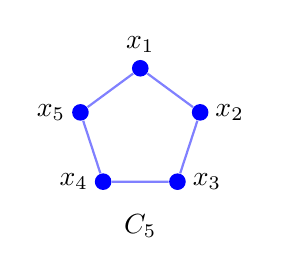
\begin{tikzpicture}[scale=0.8, vertex/.style={minimum width=6pt, circle,fill=blue, inner sep=0pt}]
\foreach \i/\x/\y in {1/0/1, 2/0.95/0.3, 3/0.59/-0.8, 4/-0.59/-0.8, 5/-0.95/0.3} {
\node[vertex] (v\i) at (\x,\y) {};
}
\node[above=2pt] at (v1){$x_1$};
\node[right=2pt] at (v2){$x_2$};
\node[right=2pt] at (v3){$x_3$};
\node[left=2pt] at (v4){$x_4$};
\node[left=2pt] at (v5){$x_5$};
\draw[blue!50,thick] (v1) -- (v2) -- (v3) -- (v4) -- (v5) -- (v1);
\node(c5) at (0,-1.5){$C_5$};
\end{tikzpicture}
\end{minipage}\hspace{3pt}
\begin{minipage}{0.23\textwidth}
\centering
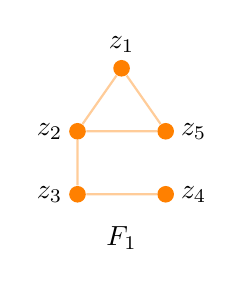
\begin{tikzpicture}[scale=0.8, vertex/.style={minimum width=6pt, circle, fill=orange, inner sep=0pt}]
\node[vertex] (z1) at (0,1){};
\node[above=2pt] at (z1) {$z_1$};
\node[vertex] (z2) at (-0.7,0){};
\node[left=2pt] at (z2) {$z_2$};
\node[vertex] (z3) at (-0.7,-1){};
\node[left=2pt] at (z3) {$z_3$};
\node[vertex] (z4) at (0.7,-1){};
\node[right=2pt] at (z4) {$z_4$};
\node[vertex] (z5) at (0.7,0){};
\node[right=2pt] at (z5) {$z_5$};
\draw[orange!40,thick](z2)--(z5)--(z1)--(z2)--(z3)--(z4);
\node at (0,-1.7){$F_1$};
\end{tikzpicture}
\end{minipage}\hspace{3pt}
\begin{minipage}{0.23\textwidth}
\centering
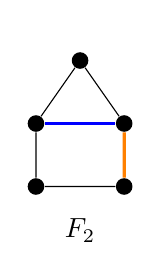
\begin{tikzpicture}[scale=0.8, vertex/.style={minimum width=6pt, circle, fill=black, inner sep=0pt}]
\node[vertex] (z1) at (0,1){};
\node[above=5pt] at (z1) {};
\node[vertex] (z2) at (-0.7,0){};
\node[vertex] (z3) at (-0.7,-1){};
\node[vertex] (z4) at (0.7,-1){};
\node[vertex] (z5) at (0.7,0){};
\draw (z5)--(z1)--(z2)--(z3);
\draw[blue, very thick](z2)--(z5);
\draw[](z3)--(z4);
\draw[orange,very thick](z4)--(z5);
\node at (0,-1.7){$F_2$};
\end{tikzpicture}
\end{minipage}
\caption{Graphs: $C_5$, $F_1$ and $F_2$ .}
\label{fig:twoc5}
\end{figure}

Table \ref{tab:computex} summarises the computed values of $\mathbb{E}[G,\alpha]$ for graphs $C_{5}$, $F_{1}$ and $F_{2}$ under  distinct 
arrival-rate vectors $\alpha$
using the 
Python code in~\cite{BFL25} , listed in the first column. For 
cycle $C_{5}$, replacing it by $F_2$ raises the expectation from $7.86$ to
$8.17$. A similar upward shift is observed
when the unicyclic graph $F_{1}$ are
augmented to $F_{2}$ (see Row 3).

\begin{table}[htbp]
\caption{$\mathbb{E}[G,\alpha]$ for $C_5$, $F_1$ and $F_2$ with arrival rates  $\alpha$ in column 1.}
\label{tab:computex}
\centering
\begin{tabular}{c|c|c|c|c}
\hline
$\alpha$ & $\mathbb{E}[G]$ & $BS(G,\alpha)$ & $\mathbb{E}[G']$ & $BS[G',\alpha]$\\
 \hline
 {1: 0.111, 2: 0.10575, 3: 0.179426, 4: 0.35046, 5: 0.253364} & 7.86 & $\{v_1,v_4\}$  & 8.17 & $\{v_1,v_4\}$ \\
 \hline
 {1: 0.266025, 2: 0.11005, 3: 0.210855, 4: 0.14145, 5: 0.27162} & 16.069 & $\{v_3,v_5\}$  & 16.89 & $\{v_3,v_5\}$ \\
 \hline
\end{tabular}
\end{table}

\subsection{$F_3$: A Star-Free Graph with Two Odd Cycles}

\begin{figure}[htbp]
\centering
\begin{minipage}{0.4\textwidth}
\centering
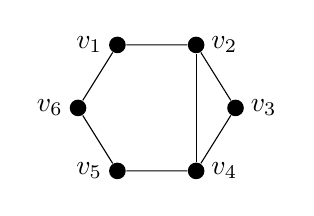
\begin{tikzpicture}[scale=1, vertex/.style={minimum width=6pt, circle, fill=black, inner sep=0pt}]
\node[vertex](v1) at (-0.5,0.8){};
\node[left=2pt] at (v1){$v_1$};
\node[vertex](v2) at (0.5,0.8){};
\node[right=2pt] at (v2){$v_2$};
\node[vertex](v3) at (1,0){};
\node[right=2pt] at (v3){$v_3$};
\node[vertex](v4) at (0.5,-0.8){};
\node[right=2pt] at (v4){$v_4$};
\node[vertex](v5) at (-0.5,-0.8){};
\node[left=2pt] at (v5){$v_5$};
\node[vertex](v6) at (-1,0){};
\node[left=2pt] at (v6){$v_6$};
\draw (v1)--(v2)--(v3)--(v4)--(v5)--(v6)--(v1);
\draw(v2)--(v4);
\end{tikzpicture}
\end{minipage}
\hspace{3pt}
\begin{minipage}{0.4\textwidth}
\centering
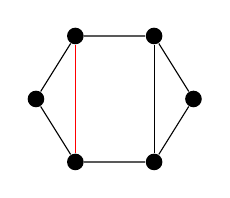
\begin{tikzpicture}[scale=1, vertex/.style={minimum width=6pt, circle, fill=black, inner sep=0pt}]
\node[vertex](v1) at (-0.5,0.8){};
\node[vertex](v2) at (0.5,0.8){};
\node[vertex](v3) at (1,0){};
\node[vertex](v4) at (0.5,-0.8){};
\node[vertex](v5) at (-0.5,-0.8){};
\node[vertex](v6) at (-1,0){};
\draw (v1)--(v2)--(v3)--(v4)--(v5)--(v6)--(v1);
\draw(v2)--(v4);
\draw[red](v1)--(v5);
\end{tikzpicture}
\end{minipage}
\caption{$F_3$ and $F_3+\{v_1,v_5\}$. }
\label{fig:twocycle}
\end{figure}
As noted previously, graph $F_3$  is obtained by inserting edge $\{v_2,v_4\}$ into graph $C_6$. The resulting star-free graph contains two distinct odd cycles with lengths $3$ and $5$, with $15$ independent sets. 
With rates $\alpha_1= 0.231787$, $\alpha_2= 0.462366$, $\alpha_3= 0.14472$, 
$ \alpha_4= 0.127484$, $\alpha_5 = 0.00342$ and $\alpha_6 =0.030223$, we get 
with the Python code described in \cite{BFL25} an expectation of total number of items equal to $39.684$ for graph $F_3$. This expectation increases to  $39.697$
when we add edge $\{v_1,v_5\}$, again a performance paradox. Both graphs have bottleneck independent set equal to 
$\{v_2,v_6\}$.


\subsection{$C_7$: Performance Paradox on a Simple Cycle}
\begin{figure}[htbp]
\centering
\begin{minipage}{0.4\textwidth}
\centering
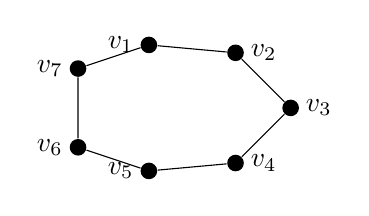
\begin{tikzpicture}[scale=1, vertex/.style={minimum width=6pt, circle, fill=black, inner sep=0pt}]
\node[vertex](v1) at (-0.5,0.8){};
\node[left=2pt] at (v1){$v_1$};
\node[vertex](v2) at (0.6,0.7){};
\node[right=2pt] at (v2){$v_2$};
\node[vertex](v3) at (1.3,0){};
\node[right=2pt] at (v3){$v_3$};
\node[vertex](v4) at (0.6,-0.7){};
\node[right=2pt] at (v4){$v_4$};
\node[vertex](v5) at (-0.5,-0.8){};
\node[left=2pt] at (v5){$v_5$};
\node[vertex](v6) at (-1.4,-0.5){};
\node[left=2pt] at (v6){$v_6$};
\node[vertex](v7) at (-1.4,0.5){};
\node[left=2pt] at (v7){$v_7$};
\draw (v1)--(v2)--(v3)--(v4)--(v5)--(v6)--(v7)--(v1);
\end{tikzpicture}
\end{minipage}
\hspace{3pt}
\begin{minipage}{0.4\textwidth}
\centering
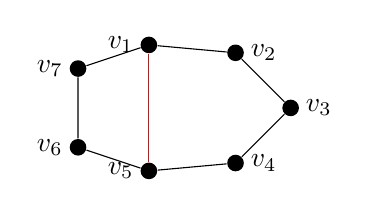
\begin{tikzpicture}[scale=1, vertex/.style={minimum width=6pt, circle, fill=black, inner sep=0pt}]
\node[vertex](v1) at (-0.5,0.8){};
\node[left=2pt] at (v1){$v_1$};
\node[vertex](v2) at (0.6,0.7){};
\node[right=2pt] at (v2){$v_2$};
\node[vertex](v3) at (1.3,0){};
\node[right=2pt] at (v3){$v_3$};
\node[vertex](v4) at (0.6,-0.7){};
\node[right=2pt] at (v4){$v_4$};
\node[vertex](v5) at (-0.5,-0.8){};
\node[left=2pt] at (v5){$v_5$};
\node[vertex](v6) at (-1.4,-0.5){};
\node[left=2pt] at (v6){$v_6$};
\node[vertex](v7) at (-1.4,0.5){};
\node[left=2pt] at (v7){$v_7$};
\draw (v1)--(v2)--(v3)--(v4)--(v5)--(v6)--(v7)--(v1);
\draw[red](v1)--(v5);
\end{tikzpicture}
\end{minipage}
\caption{$C_7$ and $C_7+\{v_1,v_5\}$. \label{fig:cycle7}}
\end{figure}

Graph $C_7$ is a simple odd cycle, with $28$ independent sets. We study
cycle graph $C_7$ together with graph $C_7+ \{v_1,v_5\}$, as illustrated in Fig.~\ref{fig:cycle7}.
Using the Python code in \cite{BFL25}, we select the arrival rate vector
$$\alpha=[{0.045206, 0.240384, 0.303789, 0.146114, 0.132526, 0.111772, 0.020209}]. 
$$
For this choice of parameters we obtain $\mathbb{E}[C_7,\alpha]=268.29593$ and  $\mathbb{E}[C_7+\{v_1,v_5\},\alpha]=285.302751$. Both graphs share the same bottleneck set $\{v_2,v_4.v_6\}$.
 
\section{(Multi)-Graph with self loops} 

Here, we assume that some 
nodes in the matching graph
have a self-loop and this was clearly forbidden by the previous assumptions in \cite{MaMo18}. Thus the compatibility graph becomes
a multigraph. 
Note that the results obtained in  \cite{MBMa21} and  \cite{MaMo18} are not valid anymore because of some technical details in 
the proofs of product form.  Such a model may represent how we can organize fair competition between players with roughly the same ranking (for instance ELO points 
for chess).  
The theory for matching models with multigraph 
has recently been presented in \cite{BMMR20} where the authors present a closed form solution for the steady-state distribution when it exists. 

\subsection{Product form on multigraphs}
Let $G=(\mathcal{V}, \mathcal{E})$ be a multigraph with the nodes partition $\mathcal{V}=\mathcal{V}_1\cup\mathcal{V}_2$ where $\mathcal{V}_1=\{i\in \mathcal{V}\mid \{i,i\}\in \mathcal{E}\}$ and $\mathcal{V}_2 = \mathcal{V}\setminus \mathcal{V}_1$. Denote by $\mathbb{I} (\check{G})$ the family of independent sets of 
$\check{G}=(\mathcal{V},\mathcal{E}\setminus\{(i,i)\mid i\in\mathcal{V}_1\})$.

\begin{theo}[Product form {\cite[Theorem 4.5]{BMMR20}}]\label{th:prod-multi}
Assume the FCFM policy and ergodicity.  
For any word $w=(w_1,\dots,w_q)\in W$,
\begin{equation}
\pi(w)= \pi({\emptyset}) \bar{\pi}(w)  =  \pi({\emptyset}) \prod_{l=1}^{q}\frac{\alpha(w_l)}{\alpha\bigl(\Gamma(\{w_1,\dots,w_l\})\bigr)},
\end{equation}
where
\[
\pi({\emptyset})^{-1}=1+\sum_{\mathcal{I}\in\mathbb{I}(\check{G})}\sum_{\sigma\in \mathfrak{S}_{|\mathcal{I}|}}
\prod_{k=1}^{|\mathcal{I}|}
\frac{\alpha(e_{\sigma(k)})}{
\alpha\bigl(\Gamma(\{e_{\sigma(1)},\dots,e_{\sigma(k)}\})\bigr)-\alpha\bigl(\{e_{\sigma(1)},\dots,e_{\sigma(k)}\}\cap \mathcal{V}_2\bigr)}. \]
\end{theo} 

 Ref \cite{BMMR20} does not provide a closed form solution for the expectation. Thus
 we develop such a formula in the following. 
For $\mathcal{I}\in\mathbb{I}(\check G)$,  fix an arbitrary ordering 
$\mathcal{I}^o=\{e_1,\dots,e_{|\mathcal{I}|}\}$. Given a permutation $\sigma$ 
of the index set $\{1,\dots,|\mathcal{I}|\}$, define the reordered 
list $\mathcal{I}^{\sigma(o)}=\{e_{\sigma(1)},\dots,e_{\sigma(|\mathcal{I}|)}\},$
that is, the sequence obtained by applying 
$\sigma$ to the ordered version $\mathcal{I}^o$. 
 We denote $\mathcal{I}_k^o$ as the first $k$ elements of $\mathcal{I}^o$.
Let $\mathcal{J}_k^o=\mathcal{I}_k^o\cap \mathcal{V}_2$. 
We define 
$$
T_{\mathcal{I}^o}=\prod_{k=1}^{|\mathcal{I}|}\frac{\alpha(e_{k})}{\alpha\Bigl(\Gamma\bigl(\mathcal{I}_k^o\bigr)\Bigr)-\alpha\Bigl(\mathcal{J}_k^o\Bigr)},
$$
and $T_{\mathcal{I}}=\sum_{\sigma \in \mathfrak{S}_{|\mathcal{I}|}} T_{\mathcal{I}^{\sigma(o)}}$. Thus $\pi(\emptyset) = (1 +T_{\mathcal{I}})^{-1}$. 
We also define
$$E_{\mathcal{I}^o}=\sum_{l=1}^{|\mathcal{I}|}
\frac{\alpha\Bigl(\Gamma\bigl(\mathcal{I}_l^o\bigr)\Bigr)}
{\alpha\Bigl(\Gamma\bigl(\mathcal{I}_l^o\bigr)\Bigr)-
\alpha\Bigl(\mathcal{J}_l^o\Bigr)}\prod_{k=1}^{|\mathcal{I}|}\frac{\alpha(e_{k})}{\alpha\Bigl(\Gamma\bigl(\mathcal{I}_k^o\bigr)\Bigr)-
\alpha\Bigl(\mathcal{I}_k^o\Bigr)},$$
and $E_{\mathcal{I}}=\sum_{\sigma \in \mathfrak{S}_{|\mathcal{I}|}} E_{\mathcal{I}^{\sigma(o)}}$.

\begin{cor}[Expectation]\label{cor:exp-multi}
The expected number of items in steady state is
\begin{equation}\label{eq:exp-multi}
\mathbb{E}[G,\alpha]=\Bigl(1+\sum_{\mathcal{I}\in\mathbb{I}(\check G)}T_\mathcal{I}\Bigr)^{-1}\sum_{\mathcal{I}\in\mathbb{I}(\check G)}E_\mathcal{I}.
\end{equation}
\end{cor} 

\begin{proof}
Clearly, 
$$
\mathbb{E}[G,\alpha]=\sum_{w\in W}|w|\,\pi(w)=
\pi_0 \sum_{w\in W}|w|\overline{\pi}(w)
=
\pi_0 \sum_{w\neq\emptyset}|w|\overline{\pi}(w).
$$ 
We now rewrite the sum over all words $w$ as a finite sum over independent sets of $\check{G}$.  For $\mathcal{I}\in\mathbb{I}(\check{G})$, let 
$\overline{\pi}_{\mathcal{I}} =\sum_{\substack{w\in W:\\ \mathrm{alphabet}(w)=\mathcal{I}}} |w|\overline{\pi}(w),$ 
where “$\mathrm{alphabet}(w)=\mathcal{I}$” means the set of distinct nodes (classes) appearing in $w$ is exactly $\mathcal{I}$.  Then $\mathbb{E}[G,\alpha]=\pi_0\sum_{\mathcal{I}\in\mathbb{I}(\check{G})}\overline{\pi}_{\mathcal{I}}$.  We claim that $\overline{\pi}_{\mathcal{I}}=E_{\mathcal{I}}$ for each independent set $\mathcal{I}\in\mathbb{I}(\check{G})$. 

Consider words $w$ whose first occurrences of the distinct letters occur in the order $i_1,\dots,i_m$.  Label the lengths between first occurrences as follows: let $p^k_l$~$(l\in\mathcal{J}_k^o)$ be the number of times letter $i_l$ appears between the first occurrence of $i_k$ (exclusive) and the first occurrence of $i_{k+1}$ (exclusive), for $l\le k$.
Let 
$n_k = \sum_{l=1}^k p^k_l $ and  $n_0=0$.
Then any such word $w$ has total length 
$|w|=|\mathcal{I}|+\sum_{k=1}^{|\mathcal{I}|} n_k$. And the multinomial coefficient is
$$\binom{n_k}{\{p_j^k\}_{j\in\mathcal{J}_k^o}}.$$
Then, we get $\overline{\pi}_{\mathcal{I}^o}$
$$
\begin{aligned}
= & \prod_{k=1}^{|\mathcal{I}|}\Bigl(\frac{\alpha({i_k})}{\alpha({\Gamma(\mathcal{I}_k^o)})}\Bigr) \sum_{n_k=0}^{\infty} \sum_{\sum p^k_j=n_k} \prod_{m=1}^k\Bigl(\frac{\alpha\bigl({i_m}\bigr)}{\alpha\bigl({\Gamma\bigl(\mathcal{I}_k^o\bigr)}\bigr)}\Bigr)^{p_m^k}\binom{n_k}{\{p_j^k\}_{j\in\mathcal{J}_k^o}}\Bigl(|\mathcal{I}|+\sum_{k=1}^{|\mathcal{I}|} n_k\Bigr) \\
= & \prod_{k=1}^{|\mathcal{I}|}\Bigl(\frac{\alpha({i_k})}{\alpha({\Gamma(\mathcal{I}_k^o)})}\Bigr) \sum_{n_k=0}^{\infty}\Bigl(\frac{\alpha({\mathcal{J}_k^o})}{\alpha\big(\Gamma\bigl(\mathcal{I}_k^o\bigr)\big)}\Bigr)^{n_k}\Bigl(|\mathcal{I}|+\sum_{k=1}^{|\mathcal{I}|} n_k\Bigr) \\
= & \sum_{l=1}^{|\mathcal{I}|} \prod_{k=1}^{|\mathcal{I}|}\Bigl(\frac{\alpha({i_k})}{\alpha({\Gamma(\mathcal{I}_k^o)})}\Bigr) \sum_{n_k=0}^{\infty}\Bigl(\frac{\alpha({\mathcal{J}_k^o})}{\alpha\big(\Gamma\bigl(\mathcal{I}_k^o\bigr)\big)}\Bigr)^{n_k}\bigl(n_l+1\bigr) \\
= & \sum_{l=1}^{|\mathcal{I}|}\Bigl(\frac{\alpha({i_l})}{ \alpha({\Gamma(\mathcal{I}_l^o)})}\Bigr) \sum_{n_l=0}^{\infty}\Bigl(\frac{\alpha({\mathcal{J}_l^o})}{ \alpha({\Gamma(\mathcal{I}_l^o)})}\Bigr)^{n_l}\bigl(n_l+1\bigr) \prod_{\substack{k \in[\![1,|\mathcal{I}|]\!]\\ k\neq l}}\Bigl(\frac{\alpha({i_k})}{\alpha({\Gamma(\mathcal{I}_k^o)}) }\Bigr)\sum_{n_k=0}^{\infty}\Bigl(\frac{ \alpha({\mathcal{J}_k^o})}{ \alpha({\Gamma(\mathcal{I}_k^o)} )}\Bigr)^{n_k} \\
= & \sum_{l=1}^{|\mathcal{I}|}\Bigl(\frac{\alpha({i_l})}{ \alpha({\Gamma(\mathcal{I}_l^o)})}\Bigr)\Bigl(\frac{ \alpha({\Gamma(\mathcal{I}_l^o)})}{ \alpha({\Gamma(\mathcal{I}_l^o)})- \alpha({\mathcal{J}_l^o})}\Bigr)^2 \prod_{{\substack{k \in[\![1,|\mathcal{I}|]\!]\\ k\neq l}}}\Bigl(\frac{\alpha({i_k})}{ \alpha({\Gamma(\mathcal{I}_k^o)})}\Bigr)\Bigl(\frac{ \alpha({\Gamma(\mathcal{I}_k^o)})}{\alpha({\Gamma(\mathcal{I}_k^o)})-\alpha({\mathcal{J}_k^o})}\Bigr) \\
= & \sum_{l=1}^{|\mathcal{I}|} \frac{\alpha({\Gamma(\mathcal{I}_l^o)})}{\alpha({\Gamma(\mathcal{I}_l^o)})-\alpha({\mathcal{J}_l^o})} \prod_{k=1}^{|\mathcal{I}|} \frac{\alpha({i_k})}{\alpha({\Gamma(\mathcal{I}_k^o)})-\alpha({\mathcal{J}_k^o})}
=E_{\mathcal{I}^o}
\end{aligned}
$$
Then, we sum over all permutation to get Equation \eqref{eq:exp-multi}.
\end{proof}

\begin{rem}
Setting $\mathcal{V}_2=\emptyset$, Theorem~\ref{th:simple} together with Corollary~\ref{cor:exp} are recovered as special instances of Theorem~\ref{th:prod-multi} and Corollary~\ref{cor:exp-multi}, respectively.
\end{rem}


\subsection{Examples of  graphs with $4$ or $7$ nodes.}\label{subsec:example}


\begin{figure}[htbp]
\centering
\begin{minipage}{0.4\textwidth}
\centering
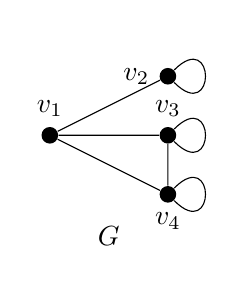
\begin{tikzpicture}[scale=0.75, vertex/.style={minimum width=6pt, circle, inner sep=0pt}]
\node at (0,-1.7){$G$};
\node[vertex,fill,label=above:$v_1$] (1) at (-1,0) {};
\node[vertex,fill,label=left:$v_2$] (2) at (1,1) {};
\node[vertex,fill,label=above:$v_3$] (3) at (1,0) {};
\node[vertex,fill,label=below:$v_4$] (4) at (1,-1) {};
\draw (2) to [out=45, in=315, loop, min distance=1cm](2);
\draw (3) to [out=45, in=315, loop, min distance=1cm](3);
\draw (4) to [out=45, in=315, loop, min distance=1cm](4);
\draw (2)--(1)--(3)--(4)--(1);
\end{tikzpicture}
\end{minipage}
\hspace{2pt}
\begin{minipage}{0.4\textwidth}
\centering
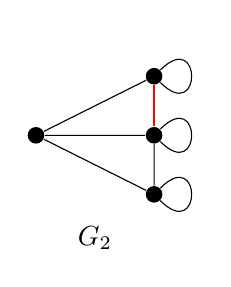
\begin{tikzpicture}[scale=0.75, vertex/.style={minimum width=6pt, circle, inner sep=0pt}]
\node at (0,-1.74){$G_2$};
\node[vertex,fill] (1) at (-1,0) {};
\node[vertex,fill] (2) at (1,1) {};
\node[vertex,fill] (3) at (1,0) {};
\node[vertex,fill] (4) at (1,-1) {};
\draw (2) to [out=45, in=315, loop, min distance=1cm](2);
\draw (3) to [out=45, in=315, loop, min distance=1cm](3);
\draw (4) to [out=45, in=315, loop, min distance=1cm](4);
\draw (2)--(1)--(3)--(4)--(1);
\draw[thick,red] (2)--(3);
\end{tikzpicture}
\end{minipage}
\caption{Graphs: $G$ and $G_2$.}
\label{fig:gandmc}
\end{figure}


\begin{figure}[htbp]
\centering
\begin{minipage}{0.45\textwidth}
\centering
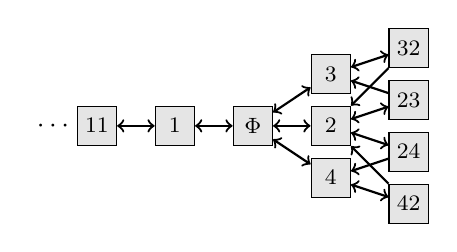
\begin{tikzpicture}[scale=0.66, state/.style={minimum width=5mm, minimum height=5mm, draw=black, fill=gray!20, inner sep=0pt, font=\footnotesize}]
\node[state] (0) at (0,0) {$\Phi$};
\node[state] (1) at (-1.5,0) {$1$};
\node[state] (11) at (-3,0) {$11$};
\node (111) at (-3.8,0) {$\cdots$};
\node[state] (3) at (1.5,1) {$3$};
\node[state] (2) at (1.5,0) {$2$};
\node[state] (4) at (1.5,-1) {$4$};
\node[state] (32) at (3,1.5) {$32$};
\node[state] (23) at (3,0.5) {$23$};
\node[state] (24) at (3,-0.5) {$24$};
\node[state] (42) at (3,-1.5) {$42$};

\draw[thick,<->](0)--(1);
\draw[thick,<->](11)--(1);
\draw[thick,<->](0)--(3);
\draw[thick,<->](0)--(2);
\draw[thick,<->](0)--(4);
\draw[thick,<->](3)--(32);
\draw[thick,<->](2)--(24);
\draw[thick,<->](2)--(23);
\draw[thick,<->](4)--(42);
\draw[thick,->](32)--(2);
\draw[thick,->](42)--(2);
\draw[thick,->](23)--(3);
\draw[thick,->](24)--(4);
\end{tikzpicture}
\end{minipage}
\vspace{2pt}
\begin{minipage}{0.45\textwidth}
\centering
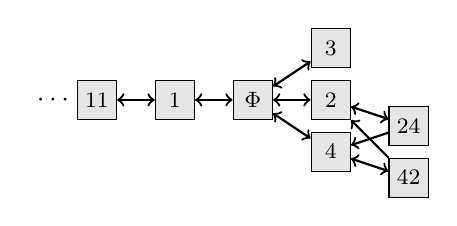
\begin{tikzpicture}[scale=0.66, state/.style={minimum width=5mm, minimum height=5mm, draw=black, fill=gray!20, inner sep=0pt, font=\footnotesize}]
\node[state] (0) at (0,0) {$\Phi$};
\node[state] (1) at (-1.5,0) {$1$};
\node[state] (11) at (-3,0) {$11$};
\node (111) at (-3.8,0) {$\cdots$};
\node[state] (3) at (1.5,1) {$3$};
\node[state] (2) at (1.5,0) {$2$};
\node[state] (4) at (1.5,-1) {$4$};
%\node[state] (32) at (3,1.5) {$32$};
%\node[state] (23) at (3,0.5) {$23$};
\node[state] (24) at (3,-0.5) {$24$};
\node[state] (42) at (3,-1.5) {$42$};

\draw[thick,<->](0)--(1);
\draw[thick,<->](11)--(1);
\draw[thick,<->](0)--(3);
\draw[thick,<->](0)--(2);
\draw[thick,<->](0)--(4);
%\draw[thick,<->](3)--(32);
\draw[thick,<->](2)--(24);
%\draw[thick,<->](2)--(23);
\draw[thick,<->](4)--(42);
%\draw[thick,red,->](32)--(2);
\draw[thick,->](42)--(2);
%\draw[thick,red,->](23)--(3);
\draw[thick,->](24)--(4);
\end{tikzpicture}
\end{minipage}
\caption{Truncation of the Markov Chains for $G$ (left) and  $G_2$ (right).}
\label{fig:mc}
\end{figure}



We consider $G=(\mathcal{V},\mathcal{E})$ in Fig.~\ref{fig:gandmc}, where $\mathcal{V}$ is partitioned into $\mathcal{V}_1=\{v_2, v_3, v_4\}$ and $\mathcal{V}_2=\{v_1\}$. The independent sets of $\check{G}$ are 
$
\{\{v_1\}, \{v_2\}, \{v_3\}, \{v_4\}, \{v_2,v_4\}, \{v_2,v_3\}\}
$.
Graph $G_2$ is 
obtained by inserting the edge $\{v_2,v_3\}$ (see Fig.~\ref{fig:gandmc}). The associated Markov Chains are depicted in Fig.~\ref{fig:mc}. 
The rates are 
$\alpha_1 = 0.432685$,$\alpha_2 = 0.005861$, $\alpha_3 = 0.141128$ and 
$\alpha_4 = 0.420326$. The BS set is a singleton (i.e. ($v1$). 
We have a paradox as the expectation slightly increases from 
$2.944793$ to $2.947256$ when we add the edge. 



The former example does not address the case of adding a new edge $e$ connecting a node lacking a self-loop to a node with self-loop. To fill this gap, we study graph $H_2$ (see Fig.\ref{fig:graphs_example2}),  obtained from $H$ by inserting edge $\{v_1,v_5\}$. Similarly, graph $H_1$ is formed by connecting $v_2$ and $v_3$, while graph $H_3$ is obtained by adding a self-loop to {$v_5$}. We have found performance paradoxes in all cases.
For arrival rate vector 
$( 0.070716, 0.180906, 0.238414, 0.204521,  0.164007, 0.07243, 
0.069006)$
the bottleneck set is $\{v_7\}$. The expectation is $31.218542$ for graph $H$ 
and it increases to 
$ 31.539906$ for graph $H_1$.  
Similarly, if we start with arrival rate vector 
$( 0.08502,  0.06418,  0.076071,  0.096493,  0.336406, 0.326572, 0.015258)$
for $H$, we get an expectation for the total number equal to $13.0179$ and the expectation is equal to $13.058815$ for the same rates and graph $H_2$. Finally, 
the comparison between $H$ and $H_3$ for rate vector $(0.104627, 0.052725,  0.194586, 0.190934, 0.117413, 0.225466,\\ 0.114249)$ also shows a performance
paradox: the expectation was $33.838547$ for $H$ and it jumps to $35.972599$ for $H_3$. In both cases, the bottleneck independent  set is singleton $\{v_6 \}$. 




\begin{figure}[htbp]
\centering
\begin{minipage}{0.22\textwidth}
\centering
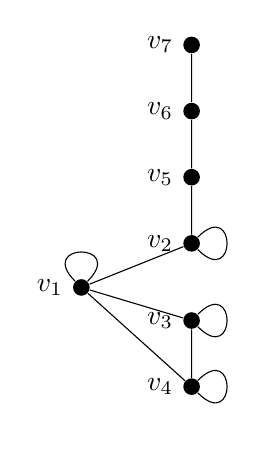
\begin{tikzpicture}[scale=0.7, vertex/.style={minimum width=6pt, circle, inner sep=0pt}]
\node[vertex,fill, label=left:$v_1$](1) at (-1,0){};
\node[vertex,fill, label=left:$v_2$](2) at (1,0.8){};
\node[vertex,fill, label=left:$v_3$](3) at (1,-0.6){};
\node[vertex,fill, label=left:$v_4$](4) at (1,-1.8){};
\node[vertex,fill, label=left:$v_5$](5) at (1,2){};
\node[vertex,fill, label=left:$v_6$](6) at (1,3.2){};
\node[vertex,fill, label=left:$v_7$](7) at (1,4.4){};
\draw (1) to [out=45, in=135, loop, min distance=1cm](1);
\draw (2) to [out=45, in=315, loop, min distance=1cm](2);
\draw (3) to [out=45, in=315, loop, min distance=1cm](3);
\draw (4) to [out=45, in=315, loop, min distance=1cm](4);
%\draw (5) to [out=45, in=315, loop, min distance=1cm](5);
\draw(1)--(3)--(4)--(1)--(2)--(5)--(6)--(7);
\end{tikzpicture}
\end{minipage}
\hspace{2pt}
\begin{minipage}{0.22\textwidth}
\centering
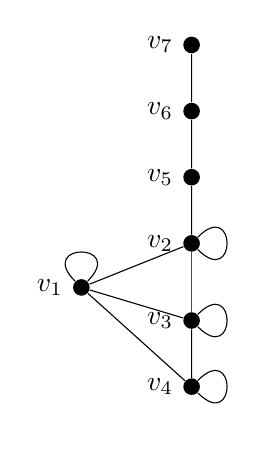
\begin{tikzpicture}[scale=0.7, vertex/.style={minimum width=6pt, circle, inner sep=0pt}]
\node[vertex,fill, label=left:$v_1$](1) at (-1,0){};
\node[vertex,fill, label=left:$v_2$](2) at (1,0.8){};
\node[vertex,fill, label=left:$v_3$](3) at (1,-0.6){};
\node[vertex,fill, label=left:$v_4$](4) at (1,-1.8){};
\node[vertex,fill, label=left:$v_5$](5) at (1,2){};
\node[vertex,fill, label=left:$v_6$](6) at (1,3.2){};
\node[vertex,fill, label=left:$v_7$](7) at (1,4.4){};
\draw (1) to [out=45, in=135, loop, min distance=1cm](1);
\draw (2) to [out=45, in=315, loop, min distance=1cm](2);
\draw (3) to [out=45, in=315, loop, min distance=1cm](3);
\draw (4) to [out=45, in=315, loop, min distance=1cm](4);
%\draw (5) to [out=45, in=315, loop, min distance=1cm](5);
\draw(1)--(3)--(4)--(1)--(2)--(5)--(6)--(7);
\draw[red] (2)--(3);
\end{tikzpicture}
\end{minipage}
\hspace{2pt}
\begin{minipage}{0.22\textwidth}
\centering
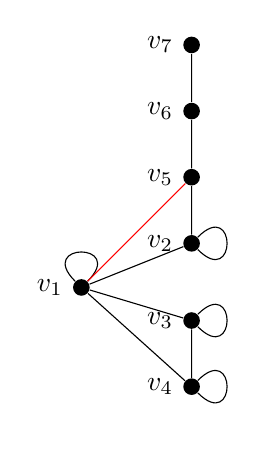
\begin{tikzpicture}[scale=0.7, vertex/.style={minimum width=6pt, circle, inner sep=0pt}]
\node[vertex,fill, label=left:$v_1$](1) at (-1,0){};
\node[vertex,fill, label=left:$v_2$](2) at (1,0.8){};
\node[vertex,fill, label=left:$v_3$](3) at (1,-0.6){};
\node[vertex,fill, label=left:$v_4$](4) at (1,-1.8){};
\node[vertex,fill, label=left:$v_5$](5) at (1,2){};
\node[vertex,fill, label=left:$v_6$](6) at (1,3.2){};
\node[vertex,fill, label=left:$v_7$](7) at (1,4.4){};
\draw (1) to [out=45, in=135, loop, min distance=1cm](1);
\draw (2) to [out=45, in=315, loop, min distance=1cm](2);
\draw (3) to [out=45, in=315, loop, min distance=1cm](3);
\draw (4) to [out=45, in=315, loop, min distance=1cm](4);
%\draw (5) to [out=45, in=315, loop, min distance=1cm](5);
\draw(1)--(3)--(4)--(1)--(2)--(5)--(6)--(7);
\draw[red](1)--(5);
\end{tikzpicture}
\end{minipage}
\hspace{2pt}
\begin{minipage}{0.22\textwidth}
\centering
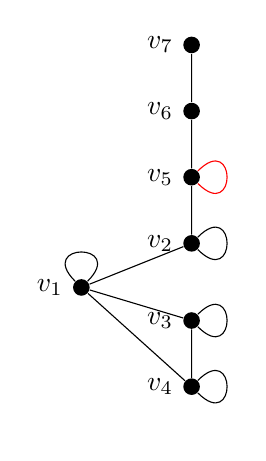
\begin{tikzpicture}[scale=0.7, vertex/.style={minimum width=6pt, circle, inner sep=0pt}]
\node[vertex,fill, label=left:$v_1$](1) at (-1,0){};
\node[vertex,fill, label=left:$v_2$](2) at (1,0.8){};
\node[vertex,fill, label=left:$v_3$](3) at (1,-0.6){};
\node[vertex,fill, label=left:$v_4$](4) at (1,-1.8){};
\node[vertex,fill, label=left:$v_5$](5) at (1,2){};
\node[vertex,fill, label=left:$v_6$](6) at (1,3.2){};
\node[vertex,fill, label=left:$v_7$](7) at (1,4.4){};
\draw (1) to [out=45, in=135, loop, min distance=1cm](1);
\draw (2) to [out=45, in=315, loop, min distance=1cm](2);
\draw (3) to [out=45, in=315, loop, min distance=1cm](3);
\draw (4) to [out=45, in=315, loop, min distance=1cm](4);
\draw[red] (5) to [out=45, in=315, loop, min distance=1cm](5);
\draw(1)--(3)--(4)--(1)--(2)--(5)--(6)--(7);
\end{tikzpicture}
\end{minipage}
\caption{graphs: $H$, $H_1$, $H_2$ and $H_3$. }
\label{fig:graphs_example2}
\end{figure}

 

\section{Conclusions and Remarks} 
This study extends the catalogue of performance paradoxes in stochastic matching models by exhibiting new star-free, sparsely connected graphs—some with self-loops—where adding a single compatibility edge or loop increases the steady-state number of waiting items. These results demonstrate that the paradox is structurally robust, arising even in small odd-cycle graphs such as $F_3$ and $C_7$. Beyond enriching the theoretical landscape, the findings caution practitioners that naive flexibility enhancements may backfire in real-world platforms. Future work should (i) characterise exact arrival-rate conditions for paradox emergence, and (ii) explore policy modifications that mitigate such counter-intuitive degradations.

\bibliographystyle{unsrt} 
\bibliography{paradoxeverywhere} 
 \end{document} 
